% !TeX program = lualatex
% !TeX TS-program = lualatex
% !BIB program = biber
% !TeX encoding = UTF-8 Unicode
%
%% This is the template to use for your master thesis Software Engineering. It
%% provides you with a structure that we expect you to follow, with guidelines on
%% the contents of each section. Depending on your research you can deviate from
%% this structure, usually by renaming or adding some chapters in the middle. Do
%% discuss this with your academic supervisor first!
%% 
%% Be sure to change the variables under the "Options" banner down below, such as
%% title, subtitle, author, examiner, company, etc., and pick a cover image (or
%% remove it entirely).
%
\RequirePackage[l2tabu, orthodox]{nag}
\documentclass[a4paper,twoside,onecolumn,openright,10pt]{mscthesis}

\usepackage{import}
\usepackage[final]{microtype}

\usepackage{polyglossia}
\setmainlanguage[variant=british]{english}
\usepackage[backend=biber,
            hyperref=true,
            isbn=true,
            backref=false,
            maxcitenames=3,
            maxbibnames=100,
            block=none,
            style=numeric-comp,
            giveninits=true,
            sortlocale=auto]{biblatex}
\addbibresource{references.bib}

\DefineBibliographyStrings{english}{%
  bibliography = {References},
  references = {References},
}

\usepackage[svgnames]{xcolor}
\usepackage{graphicx}
\graphicspath{{./figures/}}
\setkeys{Gin}{width=0.9\linewidth}
\usepackage{pgfplots}
\usepackage{tikz}
\usetikzlibrary{arrows.meta,positioning,fit}
\pgfplotsset{compat=1.18}
\usepackage{subcaption}
\captionsetup{margin=1pt}

\usepackage{xurl}
\usepackage[colorlinks=false,
			pdfborder={0 0 0},
			pdfusetitle]{hyperref}
\urlstyle{same}

\usepackage{booktabs} % publication quality tables
\usepackage{tabularx}
\usepackage{pdflscape}
\usepackage{longtable}
\usepackage{mathtools} % mathematical tools to use with amsmath
\usepackage{cleveref} % intelligent cross-referencing
\usepackage[british,xlatin,abbreviations]{foreign} % systematic treatment of 'foreign' words in documents

\usepackage[shortlabels,inline]{enumitem} % control layout of itemize, enumerate, description
\setlist{noitemsep} % shorten space between items

\settocdepth{subsection}
\setsecnumdepth{subsection}

% Change table numbers to lininig instead of oldstyle
\usepackage{etoolbox}
\AtBeginEnvironment{tabular}{\addfontfeatures{Numbers={Lining}}}

%---------------------------------------------------------------------%
%                     Options                                         %
%---------------------------------------------------------------------%

\title{Streaming Communication for Scalable Policy-Aware Data Exchange Systems}
\subtitle{A DYNAMOS Case Study}
\date{June 2026}
\author{Ruben Stoop}

% Provide the logo and address of the host organisation (company or research group)
\hostorganisation{msc-se-logo-small-white.png}{%
Complex Cyber-Infrastructure (CCI)\\
University of Amsterdam\\
Amsterdam, The Netherlands
}

% Optional cover picture. Put this in comments when not needed.
% \coverpicture{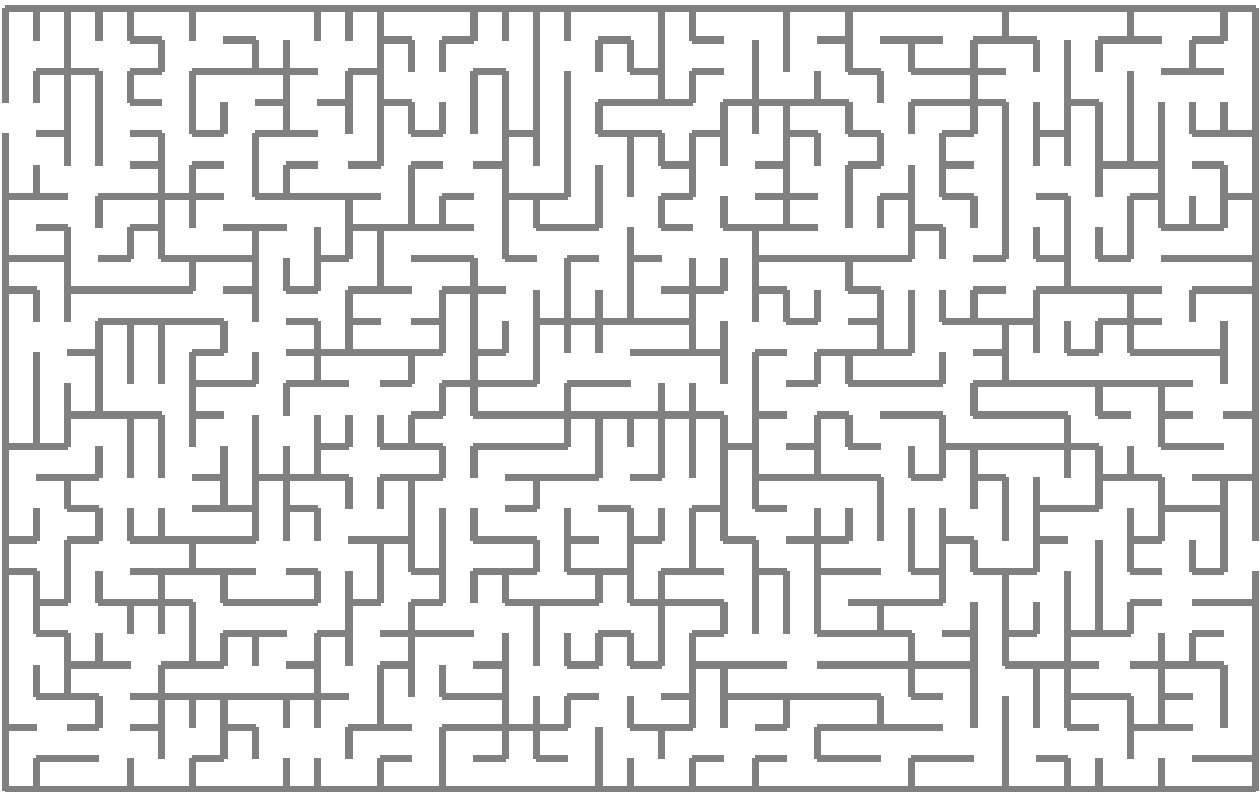
\includegraphics[width=\textwidth]{maze.pdf}}

% -- Thesis committee --

% MANDATORY
% Examiner (academic supervisor), also chair of the committee 
\examiner{Dr.\ Ana Oprescu}{CCI, UvA}
% Second reviewer (reader)
\reviewer{To be confirmed}{}

% OPTIONAL
% Daily supervisor is supervisor from a research group, typically a PhD student or Postdoc.
\dailysupervisor{Alexandros Koufakis}{CCI, UvA}
% External supervisor is the (daily) supervisor from the company
% \externalsupervisor{}{}
% Any other committee members and their affiliation
% \othermembers{}

% A copyright notice and maybe something about the cover picture.
% Put in comments to get the default copyright notice.
\colophon{\noindent{}%
  Copyright \copyright{} \theauthor{}, \the\year{}.}

%---------------------------------------------------------------------%
%                     /Options                                        %
%---------------------------------------------------------------------%

\begin{document}
%
% FRONTMATTER
%

\frontmatter
% from memdesign.pdf, see Table 2.1: Front matter
% cover title - recto, no folio
\import{frontmatter/}{cover.tex}

% title page - recto
\cleartorecto{}
\import{frontmatter/}{title.tex}

% dedication / epigraph - recto
% \cleartorecto{}
% \import{frontmatter/}{epigraph.tex}

% abstract
\cleartorecto{}
\chapter{Abstract}
\import{frontmatter/}{abstract.tex}

% blank - verso
% ToC
\cleartorecto{}
\tableofcontents{}
\clearpage{}

% List of Figures - recto or verso
\listoffigures{}
\clearpage{}

% List of Tables - recto or verso
\listoftables{}
\clearpage{}

% acknowledgments (any acknowledgemnts not mentioned in preface)
\cleartorecto{}
\chapter{Acknowledgements}
\import{frontmatter/}{acknowledgement.tex}


\mainmatter

\import{chapters/}{introduction.tex}
\import{chapters/}{background.tex}
\import{chapters/}{related_work.tex}
\import{chapters/}{methods.tex}
\import{chapters/}{experiments.tex}
\import{chapters/}{dynamos_integration.tex}
\import{chapters/}{dynamos_evaluation.tex}
\import{chapters/}{evaluation.tex}
\import{chapters/}{conclusion.tex}

%
% APPENDICES
%

\appendix

\import{appendix/}{appendix.tex}
\clearpage

%
% BACKMATTER
%

\backmatter

% Bibliography
\printbibliography{}
\cleardoublepage{}

% Acronyms
\chapter{Acronyms}
\begin{center}
\begin{tabular}{@{}lp{0.68\textwidth}@{}}
\toprule
Acronym & Meaning \\
\midrule
API & Application Programming Interface \\
CCI & Complex Cyber-Infrastructure \\
CPU & Central Processing Unit \\
DYNAMOS & Dynamically Adaptive Microservice-based Operating System \\
GC & Garbage Collection \\
gRPC & gRPC Remote Procedure Calls \\
HTTP & Hypertext Transfer Protocol \\
IEEE & Institute of Electrical and Electronics Engineers \\
IPC & Inter-Process Communication \\
ISO & International Organization for Standardization \\
JVM & Java Virtual Machine \\
JSON & JavaScript Object Notation \\
NDJSON & Newline Delimited JSON \\
REST & Representational State Transfer \\
RPC & Remote Procedure Call \\
RQ & Research Question \\
SOTA & State of the Art \\
TTP & Trusted Third Party \\
UvA & University of Amsterdam \\
VFL & Vertical Federated Learning \\
\bottomrule
\end{tabular}
\end{center}

\cleardoublepage{}

\end{document}
